\section{Characteristics}

MIPS embodies the principles of Reduced Instruction Set Computer (RISC) architecture, focusing on streamlined execution by employing simple instructions within a condensed basic cycle. 
This design aims to enhance the efficiency of Complex Instruction Set Computer (CISC) CPUs.

As a load-store architecture, MIPS operates such that Arithmetic Logic Unit  operands are sourced exclusively from the CPU's general-purpose registers, precluding direct retrieval from memory. 
Dedicated instructions are thus essential for:
\begin{itemize}
    \item Loading data from memory into registers.
    \item Storing data from registers into memory.
\end{itemize}

A pipeline architecture is a pivotal technique aimed at performance optimization. 
It capitalizes on the concurrent execution of multiple instructions derived from a sequential execution flow.

Furthermore, the Instruction Set Architecture (ISA) of MIPS encompasses a defined set of operations, instruction formats, supported hardware data types, named storage, addressing modes, and sequencing protocols.
\begin{figure}[H]
    \centering
    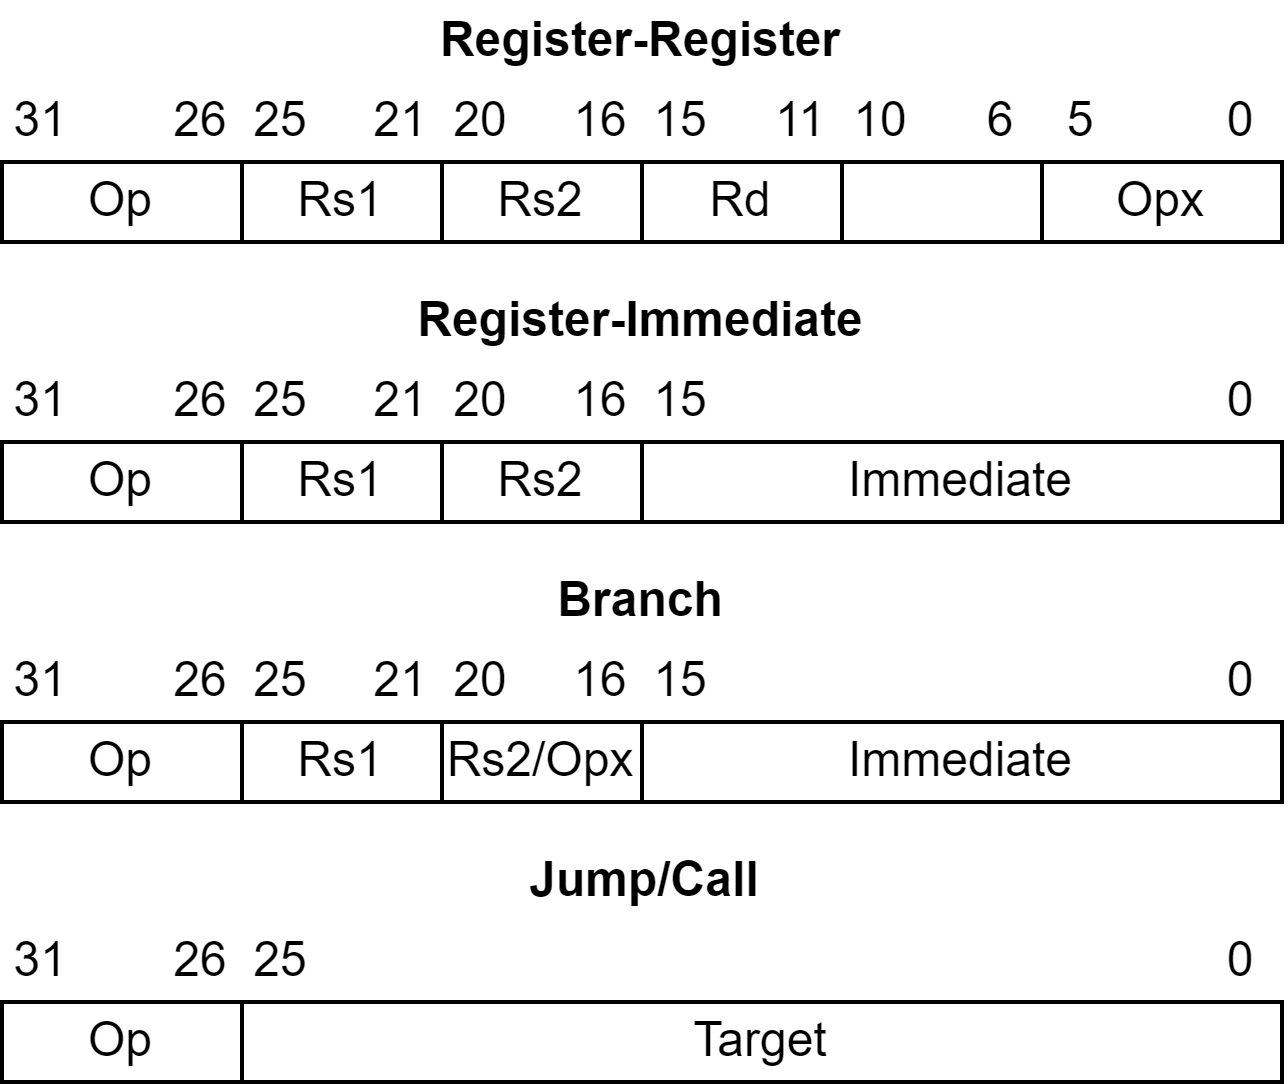
\includegraphics[width=0.4\linewidth]{images/isa.png}
    \caption{MIPS instruction set architecture}
\end{figure}

\subsection{MIPS CPU}
Within a MIPS CPU, the datapath encompasses the necessary components such as storage, functional units (FUs), and interconnects to execute desired operations effectively. 
In this setup, control points serve as inputs while signals serve as outputs.

The controller, functioning as a state machine, coordinates the activities within the datapath by directing operations based on the desired function and the signals received.
\begin{figure}[H]
    \centering
    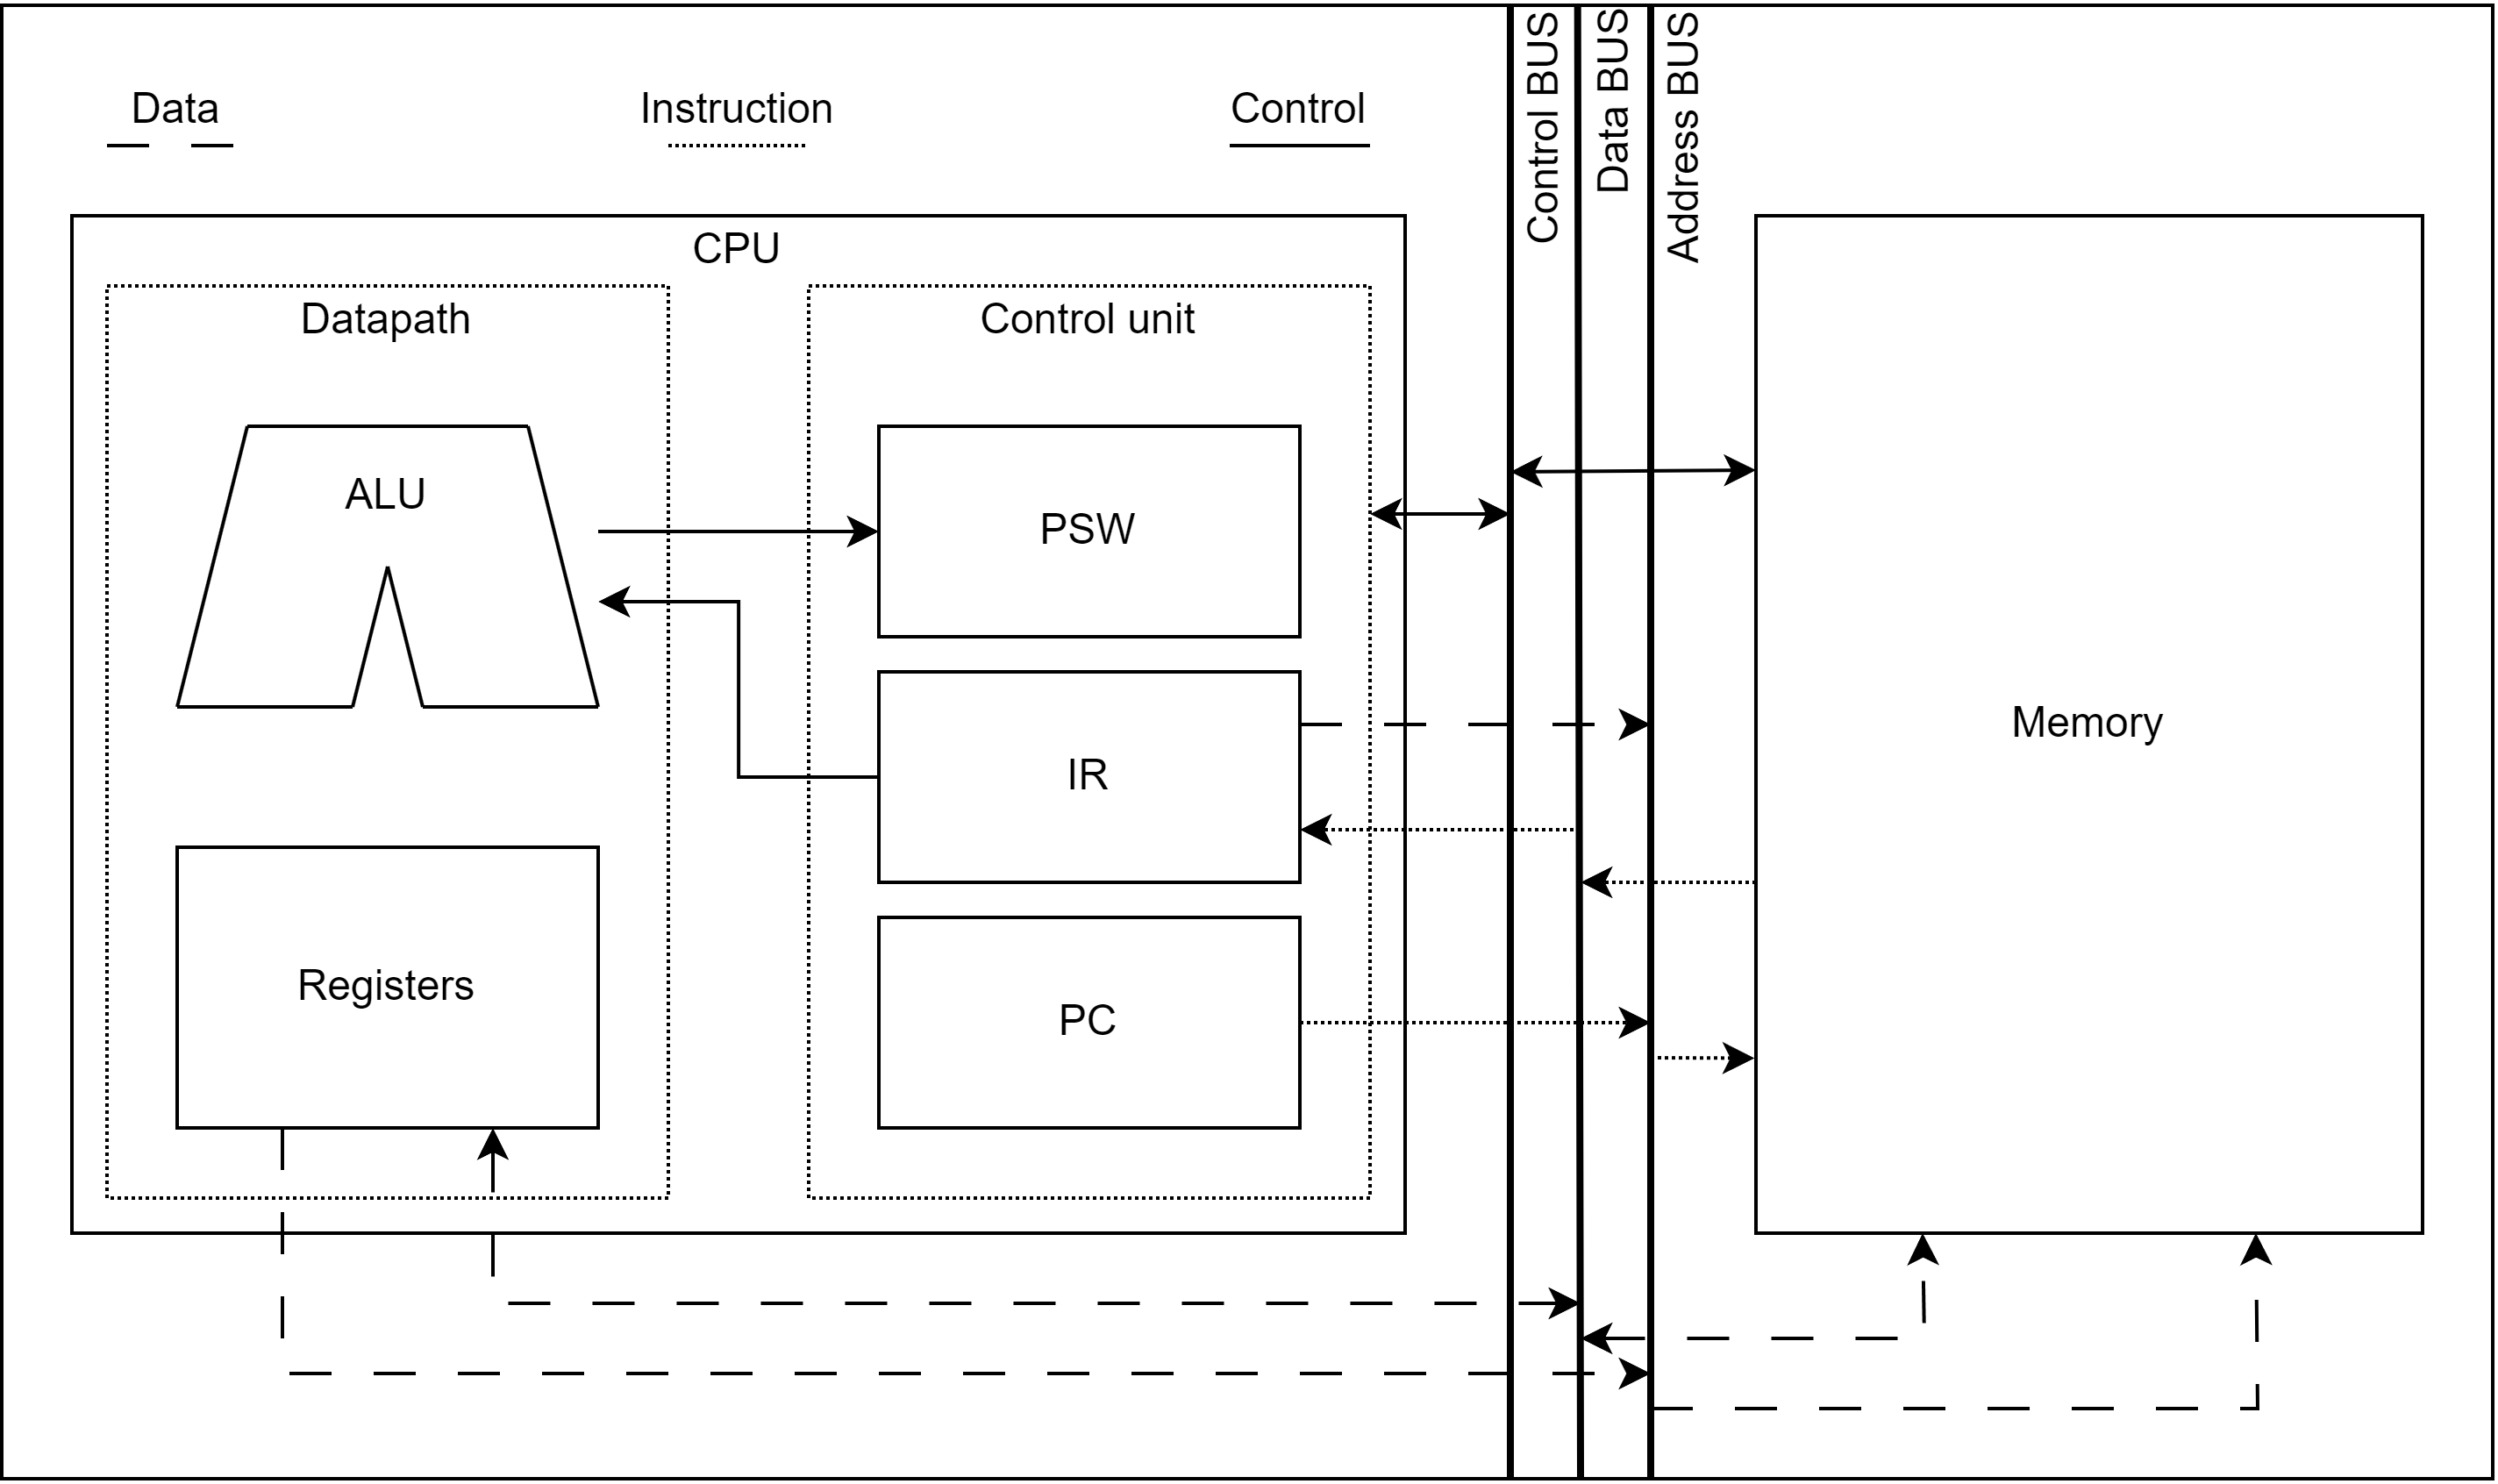
\includegraphics[width=0.75\linewidth]{images/cpu.png}
    \caption{MIPS CPU}
\end{figure}

\subsection{Program execution}
At the core, a program is segmented into instructions, with the hardware focusing on individual instructions rather than the entire program. 
At a lower level, the hardware divides instructions into clock cycles, with lower-level state machines transitioning states with each cycle.